\documentclass{article}
% if you need to pass options to natbib, use, e.g.:
     \PassOptionsToPackage{numbers, compress}{natbib}
% before loading neurips_2020

% ready for submission
% \usepackage{neurips_2020}

% to compile a preprint version, e.g., for submission to arXiv, add add the
% [preprint] option:
%     \usepackage[preprint]{neurips_2020}

% to compile a camera-ready version, add the [final] option, e.g.:
%     \usepackage[final]{neurips_2020}

% to avoid loading the natbib package, add option nonatbib:
     \usepackage[nonatbib]{neurips_2020}

\usepackage[utf8]{inputenc} % allow utf-8 input
\usepackage[T1]{fontenc}    % use 8-bit T1 fonts
\usepackage{hyperref}       % hyperlinks
\usepackage{url}            % simple URL typesetting
\usepackage{booktabs}       % professional-quality tables
\usepackage{amsfonts}       % blackboard math symbols
\usepackage{amssymb}
\usepackage{nicefrac}       % compact symbols for 1/2, etc.
\usepackage{microtype}      % microtypography
\usepackage{amsmath}
%Graphs
\usepackage{multirow}
\usepackage{tikz}
\usepackage{pgfplots}
\usepackage[export]{adjustbox}
\usepackage{xcolor,colortbl}
\usepackage[capposition=top]{floatrow}
\hypersetup{
	colorlinks,
	linkcolor = {red!50!black},
	citecolor = {blue!50!black},
	urlcolor = {blue!80!black}
}

\usepackage{lscape}
\usepackage{longtable}
\usepackage{placeins}
\usepackage{floatrow}

\title{Evaluation of Machine Learning in Empirical Asset Pricing}

% The \author macro works with any number of authors. There are two commands
% used to separate the names and addresses of multiple authors: \And and \AND.
%
% Using \And between authors leaves it to LaTeX to determine where to break the
% lines. Using \AND forces a line break at that point. So, if LaTeX puts 3 of 4
% authors names on the first line, and the last on the second line, try using
% \AND instead of \And before the third author name.

\author{%
  David S.~Hippocampus\thanks{Use footnote for providing further information
    about author (webpage, alternative address)---\emph{not} for acknowledging
    funding agencies.} \\
  Department of Computer Science\\
  Cranberry-Lemon University\\
  Pittsburgh, PA 15213 \\
  \texttt{hippo@cs.cranberry-lemon.edu} \\
  % examples of more authors
  % \And
  % Coauthor \\
  % Affiliation \\
  % Address \\
  % \texttt{email} \\
  % \AND
  % Coauthor \\
  % Affiliation \\
  % Address \\
  % \texttt{email} \\
  % \And
  % Coauthor \\
  % Affiliation \\
  % Address \\
  % \texttt{email} \\
  % \And
  % Coauthor \\
  % Affiliation \\
  % Address \\
  % \texttt{email} \\
}


%% Macros
\newcommand{\z}[2]{z_{#1, #2}}
\newcommand{\xbf}{\mathbf{x}}
\newcommand{\zVec}[3]{\mathbf{z}_{#1, #2:#3}}
\newcommand{\xVec}[3]{\mathbf{x}_{#1, #2:#3}}
\newcommand{\hVec}{\mathbf{h}}

\begin{document}

\maketitle

\begin{abstract}
	Several recent studies have claimed that machine learning methods provide superior predictive accuracy of asset returns, relative to simpler modelling approaches, and can correctly identify factors needed to price portfolio risk. Herein, we demonstrate that this performance is critically dependent on several features of the data being analysed; including, the training/test sample split, the frequency at which the data is observed, and the chosen loss-function. In contrast to existing studies, which claim that neural nets provide superior predictive accuracy, through a series of realistic examples that mimics the stylized facts of asset returns, we demonstrate that neural methods are easily outperformed by simpler methods, such as random forests and elastic nets.
\end{abstract}

\section{Introduction}
The dominance of machine learning (hereafter, ML) methods in terms of predictive accuracy has now begun to filter into the empirical asset pricing literature. The most common application of machine learning methods within finance are for portfolio construction, asset price prediction, and factor selection. 

Several studies have now used ML techniques to analyze the cross-section of asset returns and produce portfolios that can capture nonlinear information in the cross-section of asset returns. \cite{moritz2016tree} use tree-based methods to understand which firm-level characteristics best predict the cross-section of stock returns, and use this information to help mitigate portfolio risk. Similarly, \cite{messmer2017deep} uses deep feedforward neural nets (DFNs) to construct portfolios and predict the returns across a cross-sections of US asset returns. However, while \cite{messmer2017deep} demonstrates that DFNs can better capture nonlinear information, no claim is made that deep learning methods are the best approach to exploit this information. 

In addition, several studies have now suggested that machine learning methods can produce better predictions of asset returns (\cite{gu_empirical_2018}, \cite{hsu_finding_2014} and \cite{feng_deep_2018}). In particular, the results of \cite{gu_empirical_2018} suggest that, in terms of predictive performance, as measured by an out-of-sample $R^2$,  tree-based methods and shallow neural nets can provide superior predictive accuracy over other machine learning methods and simpler model-based approaches. This finding is born out both in terms of simulated data, and an empirical example with monthly returns data from 1957 to 2016. \cite{gu_empirical_2018} attribute this to machine learning's ability to evaluate and consider non-linear complexities among factors that cannot be feasibly achieved using traditional techniques. 

Similarly, work by \cite{kozak_shrinking_2017}, \cite{freyberger_dissecting_2017}, \cite{feng_taming_2019} and \cite{rapach_forecasting_2013}, demonstrate that machine learning methods can ``systematically evaluate the contribution to asset pricing of any new factor'' used within an existing linear asset pricing structure. In addition, \cite{gu_empirical_2018} use variable importance metrics to quantify the differential impact of factors across a large set of possible factors available for asset pricing. As such, these authors argue that ML can be used, \textit{en masse}, to consistently evaluate the ability of various factors to help price portfolio risk. Such work is particularly pertinent given the literature's obsession with constructing such factors: as of 2014, quantitative trading firms were using 81 factor models (\cite{hsu_finding_2014}), while \cite{harvey_census_2019} currently document that well over 600 different factors have been suggested in the literature. 

The above studies all demonstrate the potential benefits of ML methods within empirical finance. However, it is unclear if the above findings generalize to: one, different training and validation periods; two, different sampling frequencies, which results in returns with significant different characteristics;  three, different loss-measures of predictive accuracy. The answer to such questions in the realm of empirical finance are particularly pertinent given that certain ML methods, including those references above, have know difficulties in dealing with data that display the stylized facts of asset returns; e.g., penalized regression and tree-based models assume a form of conditional independence that is clearly violated by the state dependence within, and across, asset returns. Moreover, training even standard types of neural networks, such as DFNs, becomes particularly difficult when data displays strong, or nonlinear, dependence (\cite{bengio_learning_1994}). 


In some ways, existing applications of ML to empirical finance have either over-looked, downplayed, or simply ignored the importance of the above (and other) issues. \cite{messmer2017deep} and \cite{feng_deep_2018} use cross validation as part of their model building procedures, destroying the temporal ordering of data. \cite{gu_empirical_2018} and \cite{messmer2017deep} produce models using training samples that end much earlier than the data sets which they ultimately produce forecasts for: in the case of Messemer (2017), the training period ends in 1981, and forecasts are produced for the most recent 30 years of data; in  \cite{gu_empirical_2018}, the training set ends in the 1970s, with predictions ultimately produced only for the period of returns from 1987-2016.  This is particularly worrying as the factors driving returns in the 1980s, are starkly different than those driving returns in, say, 2001 onward. However, both papers suggest that their training/validation split does not impact the test set results. 

The goal of this paper is to provide a systematic, and reproducible study on the ability of ML methods to 1) accurately detect significant factors; and 2) accurately predict returns according to a range of loss measures. It is our belief that any such study is necessary in order for practitioners to reliably apply these methods in their problems of interest. 

After stating the general setup in Section two, in Section three we conduct a rigorous simulation study, which captures the stylized facts of asset returns, we give an in-depth comparison of several machine learning methods used in the literature. The simulation study explores how persistence in features, cross sectional correlation and different complexities of data generating process affect ML method's ability to: 1) accurately predict future returns across a range of loss measures; and 2) correctly identify the significant factors driving returns. In contrast to existing findings, in this realistic simulation design, we find that neural network procedures, such as feedforward nets, LSTM (CITE), and DeepAR models (CITE), are among the worst performing methods, while simpler tree-based methods and elastic net are among the best performing methods. This result is consistent across various levels of volatility, cross-sectional correlation, return signal, and different loss functions. Elastic net and tree-based methods also outperform other methods in correctly identifying significant factors.     

In Section four, the above findings are then validated via an empirical exercise that considers quarterly individual returns data from CRSP for all firms listed in the NYSE, AMEX and NASDAQ. The starting period of the data is January first 1957 (starting date of the S\&P 500) and the ending date is December 2016, totalling 60 years. A set of 549 possible factors are used to explain the cross-section of returns. We pay careful attention to the training and test split, and only use the last fourteen years of quarterly returns to evaluate the different machine learning methods. The results in this analysis completely agree with those in the aforementioned simulation study: across all machine learning methods, neural net based procedure perform the worst, while tree-based methods and elastic net perform the best. 


The results of this study suggest that great care and diligence is required if one wishes to implement machine learning methods within empirical finance. Our results suggest that the efficacy of machine learning methods within empirical finance depends on several features of the underlying problem, such as sampling frequency, the particular test training split, and the data period under analysis. As such, while potentially useful, ML methods are not a panacea for predicting, or understanding the factors that drive, financial returns. 


\section{Model and Methods}
\subsection{Statistical Model}
In this section we briefly discuss the statistical model considered for asset returns. Excess monthly returns on asset $i$, $i=1,\dots,n$, at time $t$, $t=1,\dots,T$, are assumed to evolve in an additive fashion:
%% In the case of LSTM and DeepAR, the expectation is conditional on z_t, not z_it (ie they try to leverage information from across the entire cross section to produce predictions)
\begin{equation}\label{eq:model}
r_{i, t+1} = E(r_{i, t+1} | \mathcal{F}_t) + \epsilon_{i, t+1},\;\;E(\epsilon_{i, t+1}|\mathcal{F}_{t})=0
\end{equation} where $\mathcal{F}_t$ denotes the observable information at time $t$, and $\epsilon_{i,t+1}$ is a martingale difference sequence (hereafter, mds). We further consider that the conditional mean of returns is an unknown function of a $P$-dimensional vector of features, assumed measurable at time $t$, such that 
\begin{equation}
E(r_{i, t+1} | \mathcal{F}_t) = g(z_{i,t})
\end{equation} 

The features, or predictors, $z_{i,t}$ are assumed to be composed of time-$t$ information, and depends only the characteristics of stock $i$. It is not assumed that all $z_{i,t}$ are present within the function $g(\cdot)$ across all $i$ units. That is, the function $g(\cdot)$ need not depend on the same $z_{i,t}$ as $i$ varies. The assumption that the information set can be characterized by the variables $z_{i,t}$ without dependence on the $j\neq i$ return units, is reasonable given that the collection of $z_{i,t}$ is rich enough. 

In what follows, we represent  the space of possible features as the Kronecker product of two pieces
\begin{equation}
\label{kronecker_equation}
z_{i,t} = x_t \otimes c_{i,t}
\end{equation}where the variables \( c_{i,t} \) represent a \( P_c \times 1 \) vector of individual-level characteristics for return \(i\), and \(x_t\) represents a $P_x \times 1$ vector of macroeconomic predictors, and $\otimes$ represents the Kronecker product. Thus, for $P = P_c\cdot P_x$, $z_{i,t}$ represents a $P \times 1$ feature space that can be used to approximate the unknown function $g(\cdot)$.

\subsection{Methods}Given features $z_{i,t}$, the goal of any machine learning method is to approximate the unknown function $g(\cdot)$ in \ref{eq:model}.  Broadly speaking, how different ML methods choose to approximate this function depends on three components:
\begin{enumerate}
	\item the model used to make predictions,\footnote{The model used by the ML method need not correspond to the statical models assumed to describe the data. Herein, our goal will not be to asses the ``accuracy'' of the statistical model, but to determine how different ML methods accurately determine the salient features of this model. }
	\item the regularization mechanism employed to mitigate over-fitting; 
	\item a loss function that penalized poor predictions. 
\end{enumerate}

%It is important to note that the model used by the ML method need not correspond to the statical models assumed to describe the data. In general, the specification of the statistical model entails uncertainty, however, the model a given ML method uses to generate prediction is known, possibly up to unknown functions. In what follows, our goal will not be to asses the ``accuracy'' of the statistical model, but to determine how different ML methods accurately determine the salient features of this model.   

To ensure the results of ML different methods will be comparable, we fix both the regularization mechanisms and loss functions used within each method, and allow only the models used for prediction to vary. This approach seeks to ensure that performances in one method, relative to another, are based on the model structure and not to some feature of how the models were fit. To this end, we first discuss points 2. and 3. above, and then briefly present the models used for our comparison. 
\paragraph{Loss functions:}The choice of loss function used to fit the ML methods is instrumental in the methods' ultimate performance. Herein, we consider two separate loss functions: Mean Absolute Error (MAE) and Mean Squared Error (MSE):
\begin{equation*}
\text{MAE} = \frac{1}{n} \sum_{j = i}^{n} |y_j - \hat{y_j}|\text{ and }
\text{MSE} = \frac{1}{n} \sum_{j = i}^{n} \left( y_j - \hat{y_j}\right) ^2,
\end{equation*}We consider both loss functions since MAE is less sensitive to outliers in the data which financial returns are known to exhibit, and which are caused by extreme market movements. Given this, we expect MAE to  produce predictive results that are more robust to such outlier events. 

\paragraph{Sample Splitting:} ML methods guard against over-fitting by emphasizing out-of-sample performance. To this end, observed data is split into ``training”, ``validation'' and ``test'' sets. Since returns data is intrinsically dependent, when constructing such a split we must consider a schema that respects this dependence structure. 

Throughout our experiments/applications, to balance computation and accuracy, we use a  hybrid ``rolling window"  and ``recursive'' approach to training/validation/test splits: for each model refit, the training set is increased by one year observations, i.e., $12$ monthly observations; the validation set is fixed at one year and moves forward (by one year) with each model refit; predictions are generated using that model for the subsequent year.

%This schema is chosen as it strikes a reasonable balance between computational complexity, and predictive accuracy, while allowing newer information to enter into, and have reasonable weight within, the subsequent predictions.  

\paragraph{Models} The remaining specification for the ML methods is the chosen model used to generate predictions. Herein, we consider a host of different models: including elastic net (\cite{zou_regularization_2005}, Random forest (\cite{breiman_random_2001}), feed-forward neural nets (XXX), LSTM (XXX), FFORMA (XXX) and DeepAR models (XXX). To keep the details as brief as possible, we give full details on each model and certain features of its implementation used in this work in the appendix. For each of the different methods, we consider two variants, one based on the MAE loss and one based on the MSE loss. 

\subsection{Model evaluation measures}
\paragraph{Predictive accuracy}

Predictive performance for individual excess returns are assessed using Mean Absolute Error (MAE), Mean Squared Error (MSE) (evaluated over the test set) and an out-of-sample $R^2$ measure. While  out-of-sample $R^2$ is a common measure, there is no universally agreed-upon definition. As such, we explicitly state the version employed herein as
\begin{align}
R^2_{OOS} &= 1 - \frac{\sum_{(i, t)\in\mathcal{T}_3}(r_{i, t+1} - \widehat{r}_{i, t+1})^2}
{\sum_{(i, t)\in\mathcal{T}_3} \left( r_{i, t+1} - \bar{r}_{i, t+1} \right) ^2}
\end{align}
where $\mathcal{T}_3$ indicates that the fits are only assessed on the test sub-sample, which is never used for training or tuning.

Since $R^2$ is based on in-sample-fit of a linear model, this measure is less meaningful for most of the ML methods considered in in this paper. However, we report this measure since this measure has also been considered in other applications of ML to empirical finance (see, e.g., Gu et al., 2019). 
\paragraph{Factor Selection}
An important aspect of empirical finance is the understanding of which features drive risk. That is, which features are explicitly represented within $z_{i,t}$ and can thus be used to help price risk using equation \ref{eq:model}. To this end, we define a simple variable importance (VI) measure to be applied across all ML methods in this research. To this end, we mirror the measure produced in \cite{gu_empirical_2018} and define $VI_j$ as the reduction in predictive $R^2$ from setting all values of predictor $j$ to 0, while holding the remaining model estimates fixed. Each $VI_j$ is then normalized to sum to 1. 

However, as $VI_j$ can sometimes be negative, we shift $VI_j$ by the smallest $VI_j$ plus a small constant, then dividing by this sum to alleviate numerical issues\footnote{This mechanism was chosen because the other popular normalization mechanism ``softmax" was observed to be unable to preserve the distances between each original $VI_j$, making discernment between each $VI_j$ difficult.}. The resulting VI measure is then. 
\begin{equation}
VI_{j, norm} = \frac{VI_j + \operatorname{min}(VI_j) + o}
{\Sigma VI_j + \operatorname{min}(VI_j) + o} \quad ; \quad o = 10^{-100}
\end{equation}

%%%%%%%%%%%%%%%%%%%%%%%%%%%%%%%%%%%%%%%%%
\section{Preliminary Analysis}
\subsection{Simulation study}
We first explore how ML methods perform in terms of prediction and factor selection for data that exhibit the stylized facts of empirical returns. We simulate according to a design which incorporates a low signal-to-noise ratio, stochastic volatility, persistence and cross-sectional correlated features. Data is generated from a latent factor volatility model for excess returns $r_{t+1}$, for $t=1, \dots, T$:
\begin{align*}
r_{i, t+1} &= 
g\left(z_{i, t}\right) + \beta_{i,t+1}v_{t+1} + e_{i, t+1}; 
\enspace z_{i, t} = \left(1, x_{t}\right)^{\prime} \otimes c_{i, t}, 
\enspace \beta_{i, t} = \left(c_{i 1, t}, c_{i 2, t}, c_{i 3, t}\right) \\ 
e_{i, t+1} &= 
\sigma_{i, t+1} \varepsilon_{i, t+1}; \\
\operatorname{log} (\sigma^2_{i,t+1}) &= 
\omega + \gamma \operatorname{log} (\sigma^2_{t}) + \sigma_{u}u;
\quad u \sim N(0, 1)
\end{align*}
where $v_{t+1}$ is a $3\times 1$ vector of errors, $w_{t+1} \sim N(0, 1)$,  $\varepsilon_{i,t+1} \sim N(0, 1)$ scalar error terms, matrix $C_t$ is an $N\times P_c$ matrix of latent factors, where the first three columns correspond to $\beta_{i,t}$, across the $1\leq i\leq N$ dimensions, while the remaining $P_c-3$ factors do not enter the return equation. The $P_x\times1$ vector $x_t$ is a $3 \times 1$ multivariate time series that captures for macroeconomic factors, and $\varepsilon_{t+1}$ is a $N\times 1$ vector of idiosyncratic errors. The parameters of these were tuned such that the annualized volatility of each return series was approximately 22\%, as is often observed empirically.
%%%%%%%%%%%%%%%%%%%%%
\paragraph{Characteristics}
We build in correlation across time among factors by drawing normal random numbers for each $1\leq i\leq N$ and $1\leq j\leq P_{c}$, according to:
\begin{equation}
\overline{c}_{i j, t} = \rho_{j} \overline{c}_{i j, t-1}+\epsilon_{i j, t} ;
\quad \rho_{j} \sim \mathcal{U} \left( 0.5, 1 \right) 
\end{equation}
We then build in cross sectional correlation:
\begin{align}
\widehat{C}_{t}&=L\overline{C}_{t} ; \quad B = LL' \\
B:&=\Lambda\Lambda' + 0.1\mathbb{I}_{n}, \quad
\Lambda_i = (\lambda_{i1}, \dots, \lambda_{i4}), \quad
\lambda_{ik}\sim N(0, \lambda_{sd}), \; k=1, \dots, 4
\end{align}
where $B$ serves as a variance covariance matrix with $\lambda_{sd}$ its density, and $L$ represents the lower triangle matrix of $B$ via the Cholesky decomposition. $\lambda_{sd}$ values of 0.01, 0.1 and 1 were used to explore increasing degrees of cross sectional correlation.
Characteristics are then normalized to be within $[-1, 1]$ for each $1\leq i\leq N$ and for $j=1, \dots, P_{c}$ via:
\begin{equation}
c_{i j, t} = \frac{2}{n+1} \operatorname{rank}\left(\hat{c}_{i j, t}\right) - 1.
\end{equation}
%%%%%%%%%%%%%%%%%%%%%%
\paragraph{Macroeconomic series}
We consider a Vector Autoregression (VAR) model for $x_{t}$, a $3 \times 1$ multivariate time series \footnote{More complex specifications for $A$ were briefly explored, but these did not have a significant impact on results.}:
\begin{flalign*}
x_{t} = Ax_{t-1}+u_t; 
\quad A = 0.95 I_3;
\quad u_t \sim N\left( \mu = (0, 0, 0)' , \Sigma = I_3
\right) 
\end{flalign*}
\paragraph{Return series}
We consider three different functions for $g(z_{i, t})$:
\begin{align}
(1)\; & g_1 \left(z_{i, t}\right)=\left(c_{i 1, t}, c_{i 2, t}, c_{i 3, t} \times x_{t}'[3,]\right) \theta_{0} \\
(2)\; & g_2 \left(z_{i, t}\right)=\left(c_{i 1, t}^{2}, c_{i 1, t} \times c_{i 2, t}, \operatorname{sgn}\left(c_{i 3, t} \times  x_{t}'[3,]\right)\right) \theta_{0} \\
(3)\; & g_3 \left(z_{i, t}\right) = \left(1[c_{i3,t}>0],c_{i 2, t}^{3}, c_{i 1, t} \times c_{i 2, t}\times 1[c_{i3,t}>0], \text{logit}\left({c}_{i3, t} \right)\right) \theta_{0}
\end{align}
where $x_{t}'[3,]$ denotes the third element of the $x_{t}'$ vector.
%%%%%%%%%%%%%%%%%%%%%%%%%
$g_1 \left(z_{i, t}\right)$ allows the characteristics to enter the return equation linearly, and $g_2 \left(z_{i, t}\right)$ and $g_3 \left(z_{i, t}\right)$ allow the characteristics to enter the return equation interactively and non-linearly. \footnote{($g_1, g_2$ correspond to the simulation design used by \cite{gu_empirical_2018}.)} $\theta^0$ was tuned such that the predictive $R^2$ was approximately 5\%.

The simulation design results in $3 \times 3 = 9$ different simulated datasets, each with $N = 200$ stocks, $T = 180$ periods and $P_c = 100$ characteristics. Each design was simulated 10 times to assess the robustness of machine learning algorithms, with the number of simulations kept low for computational feasibility. We employ the hybrid data splitting approach with a training:validation length ratio of approximately 1.5 and a test set that is 1 year in length. 

%% Other schemes in the forecasting literature such as using an ``inner" rolling window validation loop to find the best hyperparameters on average, finally aggregating them in an ``outer" loop for a more robust error were considered but not implemented for a variety of reasons. Firstly, many of the models were computationally too intensive for this to be feasible. More importantly, during the model fitting process it was observed that the optimal hyperparameters for the different rolling windows were highly unstable (see Appendix). Thus, this would have made the selection of the best hyperparameters on average across all windows significantly less meaningful.

%%%%%%%%%%%%%%%%%%%%%%%%%%%%%%%%%%%%%%%%%%%%%%%%%%%%%%%%%%%%%%%%%%%%%%%%%%%%%%%%%%%%%%%%%%%%%%%%%%%%%%%%%%%%%%%%%%
\subsubsection{Simulation Study Results}

\paragraph{Prediction Performance:}
An extensive discussion of the results are given in Appendix, X. For the sake of brevity, we only highlight the main results of the analysis in Table. In contrast to existing studies, we find that elastic nets are the best performing model, followed closely by random forests, then neural networks. Interestingly, all machine learning models were unaffected by the level of cross-sectional correlation in terms of prediction performance, and typically had better performance when fitted with respect to quantile loss. Random forests only outperformed the elastic nets on highly non-linear specifications. The neural network models were not observed to outperform any of the machine learning models. 


Generally, ML models fitted with respect to minimizing MAE (quantile loss) generally perform better, even when evaluated against MSE loss metrics. Though the actual level difference between the loss metrics across the penalized linear models, random forests and neural networks is small, the results are consistent across the various Monte Carlo specification. 
\begingroup\fontsize{6}{8}\selectfont

\begin{longtable}[t]{cccccccc}
\caption{\label{tab:}Top Models in Simulation Study}\\
\toprule
\multicolumn{1}{c}{ } & \multicolumn{1}{c}{ } & \multicolumn{3}{c}{Test MAE} & \multicolumn{3}{c}{Test MSE} \\
\cmidrule(l{3pt}r{3pt}){3-5} \cmidrule(l{3pt}r{3pt}){6-8}
Corr & model & g1 & g2 & g3 & g1 & g2 & g3\\
\midrule
\endfirsthead
\caption[]{Top Models in Simulation Study }\\
\toprule
\multicolumn{1}{c}{ } & \multicolumn{1}{c}{ } & \multicolumn{3}{c}{Test MAE} & \multicolumn{3}{c}{Test MSE} \\
\cmidrule(l{3pt}r{3pt}){3-5} \cmidrule(l{3pt}r{3pt}){6-8}
Corr & model & g1 & g2 & g3 & g1 & g2 & g3\\
\midrule
\endhead
\
\endfoot
\bottomrule
\endlastfoot
 & ELN.MAE & 0.0345786 & 0.0361950 & 0.0353345 & 0.0025652 & 0.0026882 & 0.0026210\\

 & RF.MAE & 0.0354594 & 0.0354204 & 0.0355399 & 0.0026434 & 0.0026305 & 0.0026446\\

 & NN2.MAE & 0.0359604 & 0.0369206 & 0.0363047 & 0.0026786 & 0.0027474 & 0.0026996\\

 & NN1.MAE & 0.0358939 & 0.0368335 & 0.0363352 & 0.0026718 & 0.0027396 & 0.0027028\\

\multirow{-5}{*}{\centering\arraybackslash \rotatebox{90}{0.01}} & NN3.MAE & 0.0358164 & 0.0369345 & 0.0364712 & 0.0026697 & 0.0027491 & 0.0027181\\
\cmidrule{1-8}
 & ELN.MSE & 0.0346142 & 0.0362761 & 0.0354437 & 0.0025676 & 0.0026980 & 0.0026300\\

 & RF.MAE & 0.0359158 & 0.0356434 & 0.0360529 & 0.0026747 & 0.0026445 & 0.0026786\\

 & NN5.MAE & 0.0370087 & 0.0372705 & 0.0374132 & 0.0027744 & 0.0027832 & 0.0027916\\

 & NN4.MSE & 0.0373820 & 0.0368966 & 0.0373542 & 0.0028051 & 0.0027505 & 0.0027970\\

\multirow{-5}{*}{\centering\arraybackslash \rotatebox{90}{1}} & NN3.MAE & 0.0372849 & 0.0370382 & 0.0371925 & 0.0027940 & 0.0027652 & 0.0027753\\*
\end{longtable}
\endgroup{}

% Across all specifications with a stochastic volatility component, we observe a decrease in prediction performance as the sample size increased according to the expanding window approach implemented. This is likely due a larger sample having a higher chance to experiences external shocks due to the stochastic volatility process, and thus a higher chance to experience large outliers in the training sample, leading to worse prediction performance. This indicates that machine learning performs poorly when the training data supplied contains more large outliers, and is still sensitive to such outliers even with the use of regularization and robust loss functions.

% Focusing on the neural networks, we clearly see that they do not outperform any of the other machine learning models, even when the underlying data generating process is non-linear. This directly contradicts the result which \cite{gu_empirical_2018} find, even when considering the design with no cross sectional correlation and stochastic volatility (top row in graphs), which corresponds to their exact specification but with a multivariate macroeconomic series. We also find consistent evidence that deeper architectures provide better prediction performance, another result which contradicts \cite{gu_empirical_2018}'s conclusions that shallow learning may be better.

\paragraph{Factor Importance}
We observe that the elastic net outperforms all other models consistently in terms of assigning the correct relative importance to the true underlying regressors, \footnote{($c_1.\text{constant}$, $c_2.\text{constant}$ and $c_3.x_3$ for $g1$ and $g_2$ specifications, and $c_1.\text{constant}$, $c_2.\text{constant}$ and $c_3.\text{constant}$ for $g_3$)} even in settings with high cross sectional correlation. 

Elastic net models perform the best at identifying the true data generating regressors, and  this appears to be mostly robust regardless of cross sectional correlation, though their performance worsens as the data generating process becomes more non-linear. On more difficult specifications, the elastic net models are conservative and typically identify a single regressor as importance - most apparent on the $g_2$ specification. Occasionally, the elastic nets identified the incorrect covariates, assigned them low relative importance.

The random forests and to a lesser extent the neural networks also correctly identified the correct underlying regressors, but struggled with adequately discerning relative importance among correlated regressors. This was became more apparent as the degree of cross sectional correlation increased (see decreasing relative importance of true underlying regressors in Figures \ref{fig:rf_sim_vi} and \ref{fig:nn_sim_vi} in Appendix). 

%% Intuitive explanation of why random forests struggle with relative discernment - not sure if necessary
%In the case of the random forests, this is to be expected, likely due to how the random forest algorithms work. The random forest algorithm is an ensemble of tree models, with each tree model only having access to a subset of all available predictors. If this subset does not include the true data generating predictor, then that particular tree will likely select the predictors which have the highest correlation with the true data generating predictor instead. Thus, the resulting ensemble model is likely to believe that cross sectionally correlated predictors are important, relative to the true underlying regressor. Due to the complexity of the neural networks, there does not exist a similar intuitive explanation for their factor selection ability.

%% Need to make these plots even smaller somehow, or omit one or two of them
%% Ended up faceting and mushing these graphs all together
\begin{figure}
	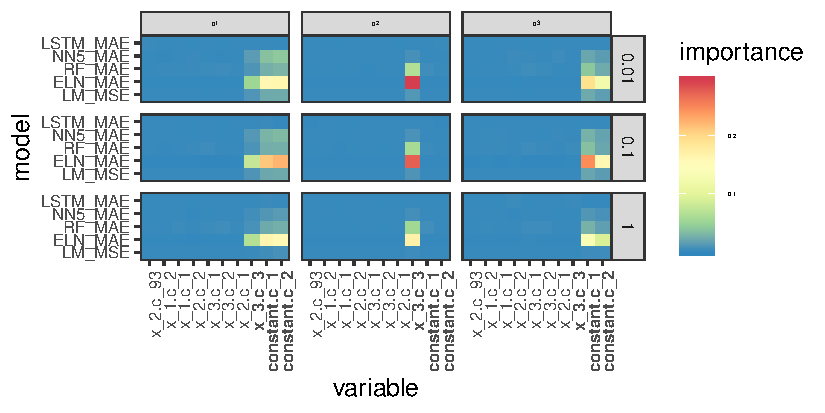
\includegraphics[max size = {\textwidth}{0.4\textheight}]{../../Results/simulation/graphics/simulation_all_g_vi.pdf}
	\caption{Simulation variable importance, faceted by simulation specification}
\end{figure}

The linear models unsurprisingly struggled with factor significance analysis with respect to both increasing cross sectional correlation non-linearities. This highlights the non-robustness and ineffectiveness of using traditional linear regression as documented by the literature; linear models were consistently observed to identify irrelevant regressors as important, especially as the degree of cross sectional correlation increased. Considering that the graphs represent the averaged variable importance metrics over different simulation realisations, this means that on a single simulation realization, the performance of linear models is significantly worse.

%% Brief other notes that are not too important

% The overall high performance of the elastic net models may be somewhat surprising given its relative simplicity compared to other machine learning models. However, when recalling that elastic net models are the only machine learning models which are specifically noted to perform well on datasets with high degrees of multicollinearity, the result is perhaps less surprising. Indeed, random forest and neural network models are only noted to be better at capturing non-linear relationships in independent and identically distributed data, a property which we observe on the non-linear specification, and only for the random forests.

% Of particular note are the instability of the machine learning models' hyperparameters across different training samples. For the elastic nets, the optimal value for $\alpha$ is generally 1 (corresponding to LASSO and thus a sparse representation), but it was not uncommon to observe $\alpha$ values swinging between values close to 0 (corresponding to ridge regression, and thus a dense representation) to 1 as the training sample moved forwards in time. As the penalized linear models consistently performed the best and still remained able to correctly identify the true covariates this is not a large issue, but it should be noted that this can lead to interpretation issues. For the random forests, it was similarly observed that the optimal value for $mtry$ (the number of variables subsetted) and $nodesize$ was highly non-robust. Again, given that the final prediction performance was consistent this is not a large issue, but can lead to some interpretation issues.

\section{Empirical analysis}
We conduct an empirical study as a final way to corroborate the findings of the properties of machine learning models which we observed in the simulation study. Though our simulation study was aimed at capturing the main features of observed data, the underlying data generating process for empirical returns is unknown. This study thus acts as a robustness check as to how machine learning performs on real world data, which can be significantly more complex and noisy than simulated contexts. 

Importantly, we find that our findings from the simulation study are largely corroborated for empirical returns data.

\subsection{Data}
We begin by obtaining monthly individual price data from CRSP for all firms listed in the NYSE, AMEX and NASDAQ, starting from 1957 (starting date of the S\&P 500) and ending in December 2016, totalling 60 years. To build individual factors, we construct a factor set based on the cross section of returns literature. This data was sourced from and is the same data used in \cite{gu_empirical_2018}. We restrict our dataset to begin from 1993 Q3 and end on 2016 Q4 to alleviate data quality issues. Our individual factor set contains 94 characteristics: 61 updated annually, 13 updated quarterly and 20 updated monthly \footnote{The dataset also included 74 Standard Industrial Classification (SIC) codes, but these were omitted due to their inconsistency, and inadequateness at classifying companies, as noted by WRDS}.

% Begin Cleaning

% the dataset was filtered such that only stocks traded primarily on NASDAQ were included (using the PRIMEXCH variable from WRDS). Then, penny stocks (also referred to as microcaps in the literature) with a stock price of less than \$5 were filtered out, as is commonly done in the literature to reduce variability. Stocks without a share code of 10 or 11 (referring to equities) were filtered out, so that securities that are not equities were not included (such as REITs and trust funds). The dataset is provided in a monthly format, which means that many of the factors which are updated only quarterly or annually have very low levels of variability, which can lead to misleading results in the model fitting process. 

We detail our cleaning procedure of this dataset. To reduce the size of the dataset and increase feasibility, we only consider non-penny equities traded primarily on the NASDAQ. To achieve a balance between having a dataset with enough data points and variability among factors, the dataset was converted to a quarterly format. Quarterly returns were then constructed using the PRC variable according to:
\begin{equation}
RET_t = (PRC_t - PRC_{t-1})/PRC_{t-1}
\end{equation}
We allow all stocks which have a quarterly return to enter the dataset, even if they disappear from the dataset for certain periods. This was primarily done to reduce survivorship bias in the dataset, and also allows for stocks which were unlisted and relisted again to feature in the dataset. \footnote{To deal with missing data, any characteristics that had over 20\% of their data missing were omitted. Remaining missing data were then imputed using their cross sectional medians for each year. See Appendix for more details.}

%% Gu et al has the missing data part as a footnote - trying that approach here

% This has the obvious drawback of introducing some bias in the dataset, as attrition in the dataset is likely to be non-random and correlated with the stocks' returns. 

% The sic2 variable, corresponding to the stocks' Standard Industrial Classification (SIC) codes was also dropped. The SIC code system suffers from inconsistent logic in classifying companies, and as a system built for pre-1970s traditional industries has been slow in recognizing new and emerging industries. Indeed, WRDS explicitly cautions the use of SIC codes beyond the use of rough grouping of industries, warning that SIC codes are not strictly enforced by government agencies for accuracy, in addition to most large companies belonging to multiple SIC codes over time. Because of this latter point in particular, there can be inconsistencies on the correct SIC code for the same company depending on the data source. Dropping the sic2 variable also reduced the dimensionality of the dataset by 74 columns, significant increasing computational feasibility.

%% Refer to table in appendix
We then follow \cite{gu_empirical_2018} and construct eight macroeconomic factors following the variable definitions in \cite{welch_comprehensive_2008} (see Table \ref{macro_factors}). These factors were lagged by one period so as to be used to predict one period ahead quarterly returns. The treasury bill rate was also used from this source to proxy for the risk free rate in order to construct excess quarterly returns. 

The two sets of factors were then combined to form a baseline set of covariates, which we define throughout all methods and analysis as:
\begin{equation}
z_{i,t} = (1, x_t)' \otimes c_{i, t}
\end{equation}
where $c_{i,t}$ is a $P_c$ matrix of characteristics for each stock $i$, and $(1, x_t)'$ is a $P_x \times 1$ vector of macroeconomic predictors, , and $\otimes$ represents the Kronecker product. $z_{i,t}$ is therefore a $P_x P_c$ vector of features for predicting individual stock returns and includes interactions between stock level characteristics and macroeconomic variables. The total number of covariates in this baseline set is $61 \times (8 + 1) = 549$\footnote{As the individual and macroeconomic factors can have similar names, individual and macroeconomic factors were prefixed with ind\_ and macro\_ respectively.}. The final dataset contains 202, 066 individual observations. We note that due to data quality issues, LSTMs, FFORMA and DeepAR are not feasible on empirical data, though the results of the simulation study suggest that even if were to be used, their performance would be underwhelming. \footnote{The dataset was not normalized for all methods, as only penalized regression and neural networks are sensitive to normalization. For these two methods, the dataset was normalized such that each predictor column had 0 mean and 1 variance.}

We mimic the sample splitting procedure used in the simulation study: the dataset was split such that the training and validation sets were split such that the training set was approximately 1.5 times the length of the validation set, in order to predict a test set that is one year in length.

\subsection{Empirical Data Results}

% Overall Results

In general, the empirical results are in remarkable agreement with the those obtained in the simulation study: the penalized linear models general perform the best, with the random forest models offering slightly worse performance. Machine learning models fitted with respect to median quantile loss were similarly observed to typically offer improvements across all machine learning models across all loss metrics. 

\paragraph{Prediction Accuracy}
In general the results of the simulation study were repeated: the elastic net models perform the best, followed by the random forests, then the DFNs, and finally the linear models. We note that the differences between each model using the MSE and MAE loss metrics are much more pronounced on empirical data. Even so, the predictive performance between the elastic net models and the quantile random forests is not particularly large, and we observe the quantile random forests outperforming the elastic nets in the first data sample. We similarly see that machine learning models perform better when fitted with respect to quantile loss instead of MSE. Most notably, we start to see the neural network models performing poorly on the empirical data, a direct contradiction to what has been reported in the literature.

%% Change this to be much smaller, fixed!
\begin{table}

\caption{\label{tab:}Top 5 models in empirical study}
\centering
\fontsize{6}{8}\selectfont
\begin{tabular}[t]{cccccccccc}
\toprule
\multicolumn{1}{c}{ } & \multicolumn{3}{c}{Sample 1} & \multicolumn{3}{c}{Sample 2} & \multicolumn{3}{c}{Sample 3} \\
\cmidrule(l{3pt}r{3pt}){2-4} \cmidrule(l{3pt}r{3pt}){5-7} \cmidrule(l{3pt}r{3pt}){8-10}
model & Test MAE & Test MSE & Test $R^2$ & Test MAE & Test MSE & Test $R^2$ & Test MAE & Test MSE & Test $R^2$\\
\midrule
ELN.MAE & 0.131369 & 0.040718 & 0.014306 & \textbf{0.137092} & \textbf{0.041892} & \textbf{0.017875} & \textbf{0.146251} & \textbf{0.045207} & \textbf{0.000835}\\
RF.MAE & \textbf{0.126703} & \textbf{0.036785} & \textbf{0.109505} & 0.173721 & 0.057546 & -0.349132 & 0.14692 & 0.046037 & -0.01752\\
NN5.MAE & 0.146411 & 0.044901 & -0.086967 & 0.18499 & 0.06461 & -0.514744 & 0.184986 & 0.063861 & -0.411475\\
NN4.MAE & 0.157301 & 0.050286 & -0.217308 & 0.168815 & 0.055711 & -0.306102 & 0.167998 & 0.055129 & -0.218463\\
NN3.MAE & 0.140781 & 0.042832 & -0.036882 & 0.181096 & 0.06216 & -0.4573 & 0.164896 & 0.053458 & -0.181528\\
\bottomrule
\end{tabular}
\end{table}

The non-robustness of DFNs is amplified on the empirical dataset. This was observed to be somewhat more common on neural networks fitted with respect to MSE, suggesting that they are indeed very sensitive to outliers in training data. We similarly observe some evidence that deeper neural networks perform better, though this result is less apparent due to the lower robustness on empirical data (see \ref{empirical_study_appendix} in Appendix for results).

% Interestingly, we do not observe worsening performance as the training sample increases as we did in the simulation study. This suggests that the simulation design may have been too volatile when compared to the specific empirical time periods examined.

\paragraph{Factor Importance}
As the data generating process for empirical returns is unknown, the variable importance results cannot be directly compared with those of the simulation study. Even so, we see similar results: the elastic net and random forest models tend to agree on the same subset of predictors, but the random forest struggles to discern between highly correlated regressors. Similar to the prediction performance results, neural networks perform poorly.

\begin{figure}[!htb]
	\centering
	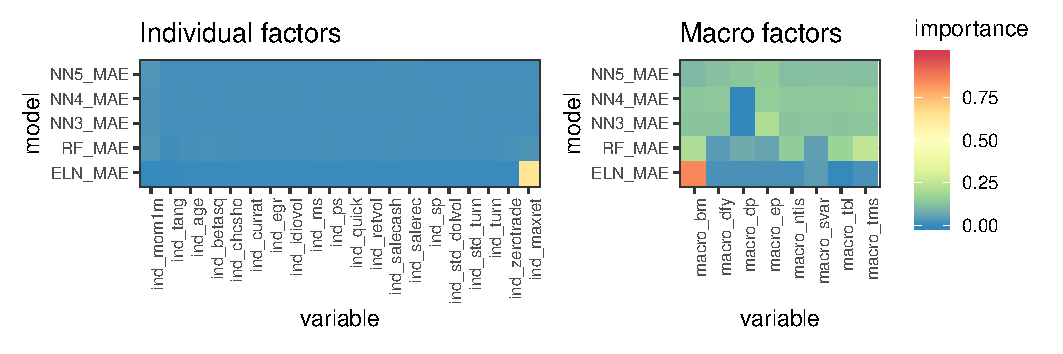
\includegraphics[max size = {\textwidth}{0.35\textheight}]{../../Results/empirical/empirical_all_sample_vi.pdf}
	\caption{Empirical individual and macroeconomic factor importance, averaged over all samples}
	\floatfoot{Individual factors shown on x axis (see Table \ref{ind_factors} in Appendix for definitions)}
\end{figure}

The elastic net, random forest and to a lesser extent DFNs tend to pick out the max return and 1 month momentum factors out of the individual characteristics as important, and the book-to-market factor out of the macroeconomic factors are important. In general, the variable importance metrics are less consistent for the random forests, and it should be noted in particular that the random forest tends to determine factors highly correlated with momentum as important, such as change in momentum, dollar trading volume and return volatility. Within the macroeconomic factors, penalized linear models tend to identify the average book to market ratio and the default spread as the most important. The random forests were inconsistent with the elastic nets, and tended to assign very similar variable importance metrics to most macroeconomic factors.

Interestingly, the linear models assign the controversial dividend price ratio macroeconomic factor as highly important, a result mirrored only with the neural networks. Their variable importance for individual factors across different training samples is non-robust, with the important variables almost completely changing year to year. The linear models consistently identified the controversial dividend-price ratio as important, a result that was somewhat consistent with the neural networks. 

The overall results again contradict the results of \cite{gu_empirical_2018}, who conclude that all of the machine methods agree on the same subset of important factors. Indeed, we only see mild consistency in variable importance between the elastic nets and random forests on the individual factors only - all other variable importance metrics were either inconsistent between different models, or non-robust.

%All models considered typically preferred sparse parameterizations. That is, most if not all of the individual factors had little to no importance across all models.\footnote{Note that because the variable importance here was not evaluated explicitly for each pairwise interaction term, some of the individual factors appear as slightly important. This is because setting an individual factor to zero also sets some of the macroeconomic pairwise terms to zero, increasing its apparent importance.}

\section{Conclusion}

Our findings demonstrate that the field of machine learning may offer certain tools to improve stock prediction and identification of true underlying factors. Penalized linear models and to a lesser extent, random forests are the best performing methods in the analysis undertaken.

Importantly, we find that DFNs fail in the context of stock return prediction, at both prediction performance and variable importance analysis. This result is consistent across a variety of simulated datasets, as well as empirical data. 

Lastly, we find that the top performing models - the elastic nets and random forests, tend to agree and correctly identify the correct underlying regressors in simulated contexts, and agree on the same subset of factors which are important in empirical contexts. We find that of all the models considered, the elastic nets are the most consistent at identifying true underlying regressors through the simulation study. We find that in the empirical setting, among the individual factors the 1 and 6 month momentum factors are the most powerful predictors of stock returns, according to the penalized linear models and random forests. 

The overall findings of this paper differ from the sparse literature on machine learning methods in empirical finance. However, the performance of the penalized linear models with respect to both out of sample prediction performance and variable importance analysis is promising, and our findings show that machine learning provides some tools which may aid in the problems of stock return prediction and risk factor selection in the financial world. 

\bibliography{Bibliography.bib}
\end{document}